\documentclass{article}
\usepackage{tikz}
\begin{document}

% TikZ Relative Coordinates Demo
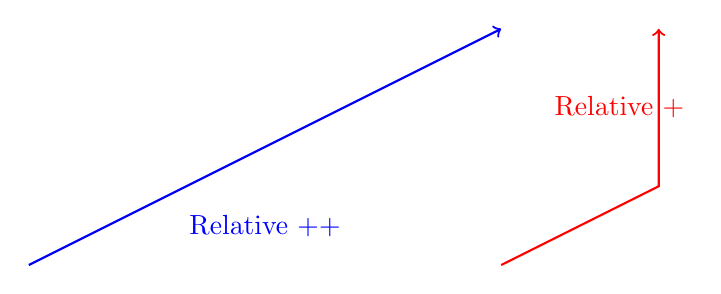
\begin{tikzpicture}[scale=1]

  % --- Using ++ (origin shifts each time) ---
  \draw[blue, thick, ->] (0,0) -- ++(2,1) -- ++(2,1) -- ++(2,1);
  \node[blue] at (3,0.5) {Relative ++};

  % --- Using + (origin stays fixed) ---
  \draw[red, thick, ->] (6,0) -- +(2,1) -- +(2,2) -- +(2,3);
  \node[red] at (7.5,2) {Relative +};

\end{tikzpicture}

\end{document}
